%% -*- mode: latex; mode:flyspell -*-
\documentclass[svgnames,x11names]{beamer}

\usepackage[british]{babel}

\usepackage{minted,tikz,tcolorbox,calc,siunitx}
\usetikzlibrary{chains,positioning,shapes.geometric,shapes.symbols,calc,shadows}
\usetikzlibrary{circuits.ee.IEC,arrows}
\usepackage{pgfplots}
\usepackage{booktabs,inconsolata}


\title{Introduction to the ARM Architecture}
\subtitle{CM0506 -- Small Embedded Systems}
\date{Lecture 3}
\author{Dr Alun Moon}
\institute{Department of Computer and Information Science}

\definecolor{NUblue}{RGB}{62,141,165}
\definecolor{NUbluedark}{RGB}{40,119,143}

\usetheme{CambridgeUS}

\usecolortheme{crane}
\setbeamercolor*{palette primary}{use=structure,fg=white,bg=NUblue}
\setbeamercolor*{palette quaternary}{fg=white,bg=NUbluedark}
\setbeamercolor{section in head/foot}{fg=white,bg=NUbluedark}
\setbeamercolor{subsection in head/foot}{fg=white,bg=NUblue}
\setbeamercolor{frametitle}{fg=NUbluedark!150,bg=NUblue!40}
\setbeamercolor{title in head/foot}{fg=white,bg=NUblue}
\setbeamercolor{author in head/foot}{fg=white, bg=NUbluedark}
\setbeamercolor{date in head/foot}{fg=white, bg=NUblue!60}
\setbeamercolor{title}{fg=NUbluedark!150,bg=NUblue!30}
\setbeamercolor{date}{fg=NUbluedark!150}
\setbeamercolor{block title}{fg=white,bg=NUblue}

\usepackage[T1]{fontenc}
\usepackage[utf8]{inputenc}

\begin{document}

\frame\maketitle

\begin{frame}{RISC/CISC Processors}{}
  \begin{block}{Complex Instruction Set Computers (\bfseries{CISC})}
    \begin{itemize}
    \item Dense code, simple compiler
    \item Powerful instruction set,
      variable format, multi word
    \item Microcoded
    \item Multi-cycle execution
    \end{itemize}
  \end{block}
  \begin{block}{Reduced Instruction Set Computers (\bfseries{RISC})}
    \begin{itemize}
    \item Small instruction set -- hardwired
    \item High clock rate, low development costs
    \item Simple instructions, fixed format, complex optimising
      compiler
    \item Many registers may be banked
    \item Smaller die
      size, lower power
    \end{itemize}
  \end{block}
\end{frame}

\begin{frame}[fragile]{Is the ARM a RISC}
  \begin{itemize}
  \item ARM has 16 GP registers (but so does the 68000) 
  \item Some ARM instructions are complex: 
\begin{verbatim}
    LDMEQFD r13!,{r0,r2-r4,pc}^ 
\end{verbatim}
  \item ARM has simple hardware with modular design 
  \item Smaller Si -- quicker to market and easier to incorporate as
    IP
  \item ARM power consumption is low -- battery operated kit, less
    cooling
  \item Most instructions executed in single cycle
  \item Access to memory is only through Load/Store instructions
  \end{itemize}
\end{frame}

\begin{frame}{ARM Design Philosophy}
  \begin{description}
  \item[Variable cycle execution] most instructions require a single
    cycle -- some are longer
  \item[Inline barrel shifter] expands many instructions -- improved
    density and performance
  \item[Thumb 16-bit instructions] improved code density for a subset
    of instructions
  \item[Conditional execution] all instructions may be conditional --
    improved performance by reducing branching and increasing code
    density
  \item[Enhanced Instructions] DSP instructions for 16x16-bit multiply
  \end{description}
\end{frame}

\begin{frame}{ARM Inside}
  ARM is one of the most popular 32-bit cores 4 billion ARM cores were
  manufactured in 2008
  \begin{columns}[onlytextwidth]
    \begin{column}{.5\textwidth}
      \begin{itemize}
      \item Gameboy consoles
      \item Set-top boxes
      \item Satellite receivers
      \item WinTV
      \item Sony minidisc
      \item Digital cameras
      \item Laser printers
      \end{itemize}
    \end{column}
    \begin{column}{.5\textwidth}
    \begin{itemize}
      \item GSM handsets
    \item Cable/ADSL modems
    \item Routers
    \item POS systems
    \item Smart cards
    \item Pocket PCs
    \item Hand-held PCs
    \item Various PDAs
    \end{itemize}
  \end{column}
\end{columns}
\end{frame}

\begin{frame}{The ARM Processor}
  \begin{itemize}
  \item First ARM processor developed in 3 micron technology in
    `83-85'
  \item This course is based on the ARM7 architecture of early 90's
  \item DEC (now Compaq) developed the high performance StrongARM
    processor
  \item Recent developments are: ARM8 and ARM9E (1999), and a ARM
    processor without a clock -- the AMULET
  \item We are using an ARM processor manufactured by NXP (Philips)
  \end{itemize}
\end{frame}

\begin{frame}{Internal Organisation of ARM7}{}
\begin{columns}[onlytextwidth]
\begin{column}{.5\textwidth}
  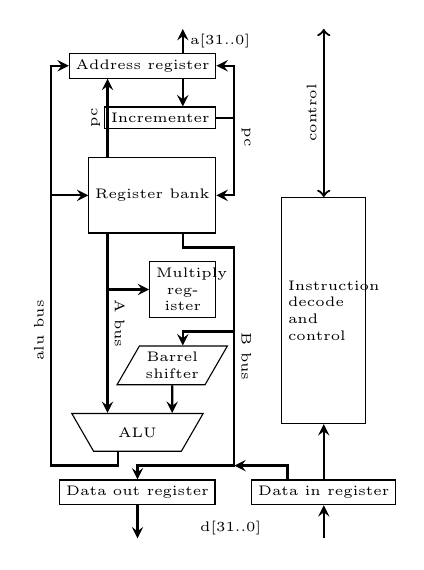
\begin{tikzpicture}[node distance=10pt,
    shifter/.style={draw,trapezium,trapezium right angle=120},
    alu/.style={draw,trapezium,
      trapezium left angle=120,
      trapezium right angle=120,
      minimum width=18ex,minimum height=2em},
    register/.style={draw,rectangle},
    bus/.style={thick,-stealth}]\tiny
    \node[register,minimum width=18ex] (address) {Address register};
    \node[register,below=of address.south east,anchor=north east]
    (incr) {Incrementer};

    \node[register,minimum width=18ex,minimum height=4em,
    below=of incr.south east,anchor=north east] (bank) {Register bank};
    \node[register,text width=9ex,align=center,below=of bank.south
    east,anchor=north east] (multiply) {Multiply register};
 
    \node[coordinate,below=of multiply.south east] (p){};
    \node[shifter,draw,right=2ex of p, align=center,anchor=top right
    corner] (shift)  {Barrel\\shifter}; 
 
    \node[coordinate,below=of shift.south east] (q){};
    \node[alu,right=2ex of q,anchor=top right corner] (alu) {ALU};
    \node[register,below=of alu] (out) {Data out register};
    \node[register,right=6ex of out] (in) {Data in register}; 

    \coordinate[left=3ex of address.west] (l) {};
    \coordinate[right=3ex of address.east] (r) {};
  
    \draw[bus] (multiply|-address.south) -- (multiply|-incr.north);
    \draw[bus] (incr) -| (r) -- (address);
    \draw[bus] (incr) -- (incr-|r) |- node[sloped,above,very near start]{pc} (bank);

    \coordinate (a1) at ($(bank.south-|multiply)!.5!(multiply.north)$);
    \coordinate (a2) at ($(shift.north-|multiply)!.5!(multiply.south)$);

    \draw[bus] (bank.south-|multiply) |- (a1-|r) |- (a2) -- (shift.north-|multiply);
    \coordinate (b1) at ($(alu.south)!.5!(out.north)$);
    \draw[bus] (a1-|r) --node[sloped,above]{B bus} (r|-b1) -| (out);

    \coordinate (c2) at ($(bank.south west)!0.3!(bank.south)$);

    \draw[bus] (c2|-bank.north) --node[sloped,above]{pc} (c2|-address.south);

    \draw[bus] (c2) --node[sloped,above]{A bus} (alu.north-|c2);
    \draw[bus] (c2) |- (multiply);

    \draw[bus] (shift) -- (shift|-alu.north);

    \draw[bus] (alu.south west) |- (b1-|l) -- node[sloped,above]{alu
      bus} (l|-bank) -- (bank);
    \draw[bus] (bank-|l) |- (address);

    \draw[bus] ($(in.north west)!.5!(in.north)$) |- (r|-b1);

    \node[draw,rectangle, text width=12ex, above=20pt of in,
    minimum height=12em] (m) {Instruction decode and\\ control};
    \draw[bus] (in) -- (m);

    \coordinate[above=4ex of address.north] (top) {};
    \draw[bus] (address.north-|multiply) --node[right]{a[31..0]} (top-|multiply);
    \draw[bus,<->] (m) -- node[sloped,above]{control} (m|-top);
    \draw[bus] (out.south) -- ++(-90:12pt);
    \draw[bus] (in.south) ++(-90:12pt) -- (in.south);
    \coordinate (d) at ($(out)!.5!(in)$);
    \node[below=8pt of d] {d[31..0]};
  \end{tikzpicture}
\end{column}
\begin{column}{.5\textwidth}
  \begin{itemize}
  \item Two main blocks: datapath and decoder
  \item Register bank (r0 to r15)
  \item Two read ports for A-bus/B-bus
  \item One write port for ALU-bus
  \item Additional read/write ports for program counter r15
  \item Barrel shifter -- shift/rotate 2nd operand by any number of bits
  \item ALU performs arithmetic/logic functions
  \item Address registers/incrementer holds PC address (with
    increment) or operand address
  \end{itemize}
\end{column}
\end{columns}
\end{frame}

\begin{frame}{ARM Instruction Format}
  \begin{itemize}
  \item 3 address format of ARM

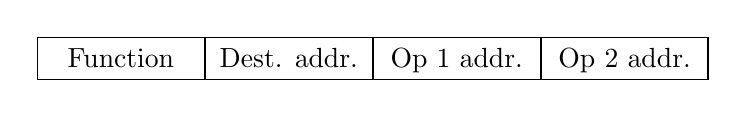
\begin{tikzpicture}[text height=1.75ex,text depth=0.25ex,minimum
  width=14ex]
  \matrix[column sep=0pt,row sep=2ex,ampersand replacement=\&] {
    \node[draw,rectangle]{Function}; \&
    \node[draw,rectangle]{Dest. addr.}; \& \node[draw,rectangle]{Op 1
      addr.}; \&
    \node[draw,rectangle]{Op 2 addr.}; \\
  };
\end{tikzpicture}

\item 2 address format of ARM Thumb instruction set 

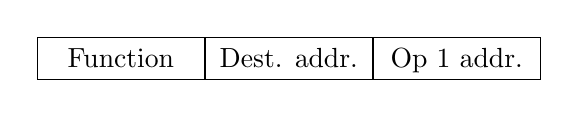
\begin{tikzpicture}[text height=1.75ex,text depth=0.25ex,minimum
  width=14ex]
  \matrix[column sep=0pt,row sep=2ex,ampersand replacement=\&] {
    \node[draw,rectangle]{Function}; \&
    \node[draw,rectangle]{Dest. addr.}; \& \node[draw,rectangle]{Op 1
      addr.}; \\
  };
\end{tikzpicture}
\end{itemize}
\end{frame}


\begin{frame}{Instruction}{Fetch/Execute cycle}
\begin{columns}[onlytextwidth]
\begin{column}{.5\textwidth}
  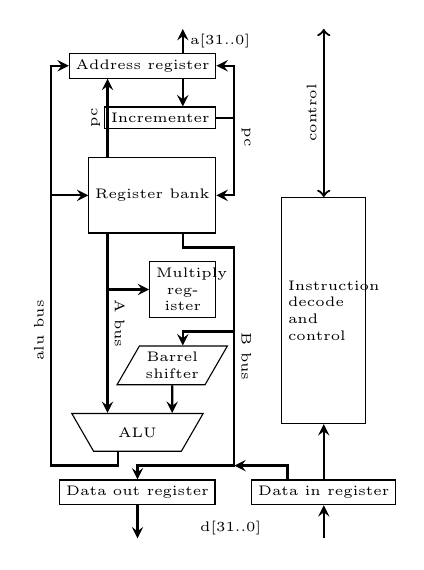
\begin{tikzpicture}[node distance=10pt,
    shifter/.style={draw,trapezium,trapezium right angle=120},
    alu/.style={draw,trapezium,
      trapezium left angle=120,
      trapezium right angle=120,
      minimum width=18ex,minimum height=2em},
    register/.style={draw,rectangle},
    bus/.style={thick,-stealth}]\tiny
    \node[register,minimum width=18ex] (address) {Address register};
    \node[register,below=of address.south east,anchor=north east]
    (incr) {Incrementer};

    \node[register,minimum width=18ex,minimum height=4em,
    below=of incr.south east,anchor=north east] (bank) {Register bank};
    \node[register,text width=9ex,align=center,below=of bank.south
    east,anchor=north east] (multiply) {Multiply register};
 
    \node[coordinate,below=of multiply.south east] (p){};
    \node[shifter,draw,right=2ex of p, align=center,anchor=top right
    corner] (shift)  {Barrel\\shifter}; 
 
    \node[coordinate,below=of shift.south east] (q){};
    \node[alu,right=2ex of q,anchor=top right corner] (alu) {ALU};
    \node[register,below=of alu] (out) {Data out register};
    \node[register,right=6ex of out] (in) {Data in register}; 

    \coordinate[left=3ex of address.west] (l) {};
    \coordinate[right=3ex of address.east] (r) {};
  
    \draw[bus] (multiply|-address.south) -- (multiply|-incr.north);
    \draw[bus] (incr) -| (r) -- (address);
    \draw[bus] (incr) -- (incr-|r) |- node[sloped,above,very near start]{pc} (bank);

    \coordinate (a1) at ($(bank.south-|multiply)!.5!(multiply.north)$);
    \coordinate (a2) at ($(shift.north-|multiply)!.5!(multiply.south)$);

    \draw[bus] (bank.south-|multiply) |- (a1-|r) |- (a2) -- (shift.north-|multiply);
    \coordinate (b1) at ($(alu.south)!.5!(out.north)$);
    \draw[bus] (a1-|r) --node[sloped,above]{B bus} (r|-b1) -| (out);

    \coordinate (c2) at ($(bank.south west)!0.3!(bank.south)$);

    \draw[bus] (c2|-bank.north) --node[sloped,above]{pc} (c2|-address.south);

    \draw[bus] (c2) --node[sloped,above]{A bus} (alu.north-|c2);
    \draw[bus] (c2) |- (multiply);

    \draw[bus] (shift) -- (shift|-alu.north);

    \draw[bus] (alu.south west) |- (b1-|l) -- node[sloped,above]{alu
      bus} (l|-bank) -- (bank);
    \draw[bus] (bank-|l) |- (address);

    \draw[bus] ($(in.north west)!.5!(in.north)$) |- (r|-b1);

    \node[draw,rectangle, text width=12ex, above=20pt of in,
    minimum height=12em] (m) {Instruction decode and\\ control};
    \draw[bus] (in) -- (m);

    \coordinate[above=4ex of address.north] (top) {};
    \draw[bus] (address.north-|multiply) --node[right]{a[31..0]} (top-|multiply);
    \draw[bus,<->] (m) -- node[sloped,above]{control} (m|-top);
    \draw[bus] (out.south) -- ++(-90:12pt);
    \draw[bus] (in.south) ++(-90:12pt) -- (in.south);
    \coordinate (d) at ($(out)!.5!(in)$);
    \node[below=8pt of d] {d[31..0]};
  \end{tikzpicture}
\end{column}
\begin{column}{.5\textwidth}
  \begin{itemize}
  \item Data register holds read/write data to/from memory Instruction
    decoder decodes machine instructions to produce control signals to
    datapath
  \item In single-cycle data processing instructions, data values are
    read on the A-bus \& B-bus, the result from the ALU is written
    back into register bank
  \item PC value in address register is incremented and copied back to
    r15 and the address register -- allowing fetching new instructions
    ahead of time (instruction pre-fetch)
  \end{itemize}
\end{column}
\end{columns}
\end{frame}

\begin{frame}{Pipelining}
  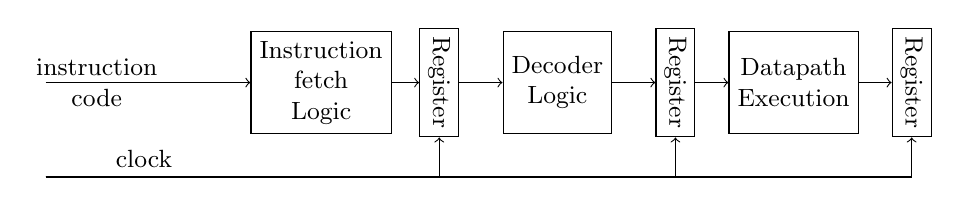
\begin{tikzpicture}[
    stage/.style={align=center,rectangle,draw,minimum
      width=10ex,minimum height=4em}
    ]\small
    \draw (-2,0) node[coordinate] (start) {};
    \draw (-2,-1.2) node[coordinate] (clock) {};
    \draw (1.5,0) node[stage] (fetch) {Instruction\\ fetch\\ Logic};
    \draw (3,0) node[draw,rectangle,rotate=-90,anchor=center] (r1) {Register};
    \draw (4.5,0) node[stage] (decode) {Decoder\\ Logic};
    \draw (6,0) node[draw,rectangle,rotate=-90,anchor=center] (r2) {Register};
    \draw (7.5,0) node[stage] (execute) {Datapath\\ Execution};
    \draw (9,0) node[draw,rectangle,rotate=-90,anchor=center] (r3)
    {Register};
    \draw[->] (start) -- node[near start,align=center] {instruction\\code} (fetch);
    \draw[->] (fetch) -- (r1);
    \draw[->] (r1) -- (decode);
    \draw[->] (decode) -- (r2);
    \draw[->] (r2) -- (execute);
    \draw[->] (execute) -- (r3);
    \draw[->] (clock) -| node[very near start,above]{clock} (r1);
    \draw[->] (clock) -| (r2);
    \draw[->] (clock) -|  (r3);
  \end{tikzpicture}
  \begin{itemize}
  \item ARM7 uses 3-stage instruction pipeline
    \begin{description}
    \item[Fetch] fetch instruction code from memory into instruction
      pipeline
    \item[Decode] instruction decoded to obtain control signals for
      the datapath ready for the next stage
    \item[Execute] instruction ``owns'' the datapath -- register read;
      shifting; ALU result generated and write-back
    \end{description}
  \item Result of each stage stored in registers
  \item The consequence is that the clock period is much shorter than
    without pipelining
  \end{itemize}
\end{frame}

\begin{frame}{Pipelining}

  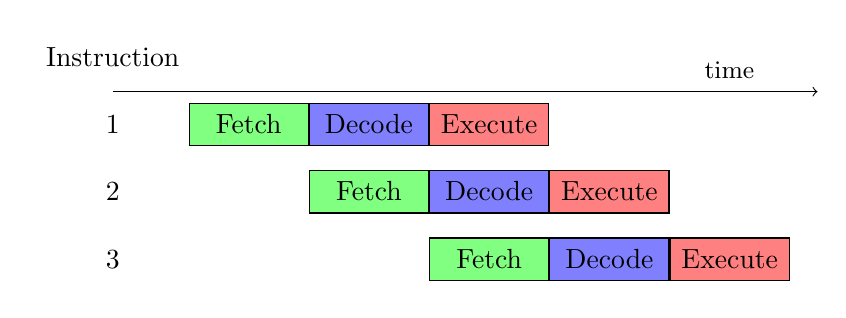
\begin{tikzpicture}[text height=1.75ex,text depth=0.25ex,minimum
    width=10ex]
    \node [matrix,column sep=0pt,row sep=2ex,ampersand replacement=\&,
        fetch/.style={draw,rectangle,fill=green!50},
        decode/.style={draw,rectangle,fill=blue!50},
        execute/.style={draw,rectangle,fill=red!50},
        ]  {
      \node (instruction) {Instruction}; \\
      \node {1}; \&
      \node[fetch]{Fetch}; \&
      \node[decode]{Decode}; \&
      \node[execute]{Execute}; \\
      \node {2}; \&
      \& \node[fetch]{Fetch}; \&
      \node[decode]{Decode};
      \& \node[execute]{Execute}; \\n
      \node {3}; \&
      \& \& \node[fetch]{Fetch}; \&
      \node[decode]{Decode}; \&
      \node[execute] (pipeline) {Execute}; \\
    } ;
    \coordinate[below=1ex of instruction.south] (Ori) {};
    \coordinate[right=1em of pipeline.east] (End) {};
    \draw[->] (Ori) --node[above,very near end]{\small time} (Ori-|End);
  \end{tikzpicture}

  \begin{itemize}
  \item At any time, 3 different instructions may occupy each of the
    3-stages of pipeline
  \item It may take three cycles to complete a single-cycle
    instruction -- a three cycle latency
  \item Once a pipeline fills, the processor completes a single cycle
    instruction every clock cycle. Therefore the throughput is one
    instruction per cycle.
  \end{itemize}
\end{frame}

\begin{frame}[fragile]{Datapath activity during data processing instruction}{}{}
\begin{columns}[onlytextwidth]
\begin{column}{.5\textwidth}
  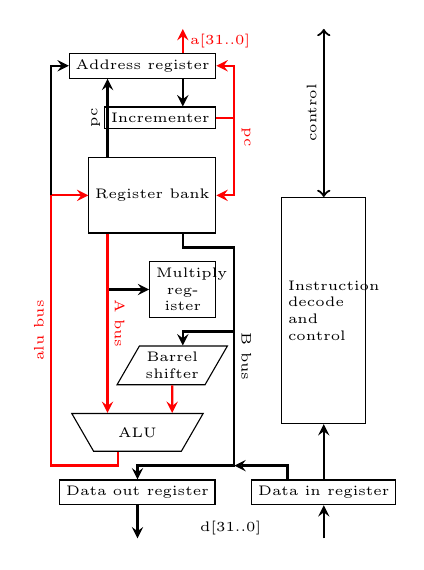
\begin{tikzpicture}[node distance=10pt,
    shifter/.style={draw,trapezium,trapezium right angle=120},
    alu/.style={draw,trapezium,
      trapezium left angle=120,
      trapezium right angle=120,
      minimum width=18ex,minimum height=2em},
    register/.style={draw,rectangle},
    bus/.style={thick,-stealth}]\tiny
    \node[register,minimum width=18ex] (address) {Address register};
    \node[register,below=of address.south east,anchor=north east]
    (incr) {Incrementer};

    \node[register,minimum width=18ex,minimum height=4em,
    below=of incr.south east,anchor=north east] (bank) {Register bank};
    \node[register,text width=9ex,align=center,below=of bank.south
    east,anchor=north east] (multiply) {Multiply register};
 
    \node[coordinate,below=of multiply.south east] (p){};
    \node[shifter,draw,right=2ex of p, align=center,anchor=top right
    corner] (shift)  {Barrel\\shifter}; 
 
    \node[coordinate,below=of shift.south east] (q){};
    \node[alu,right=2ex of q,anchor=top right corner] (alu) {ALU};
    \node[register,below=of alu] (out) {Data out register};
    \node[register,right=6ex of out] (in) {Data in register}; 

    \coordinate[left=3ex of address.west] (l) {};
    \coordinate[right=3ex of address.east] (r) {};
  
    \draw[bus] (multiply|-address.south) -- (multiply|-incr.north);
    \draw[bus,red] (incr) -| (r) -- (address);
    \draw[bus,red] (incr) -- (incr-|r) |- node[sloped,above,very near start]{pc} (bank);

    \coordinate (a1) at ($(bank.south-|multiply)!.5!(multiply.north)$);
    \coordinate (a2) at ($(shift.north-|multiply)!.5!(multiply.south)$);

    \draw[bus] (bank.south-|multiply) |- (a1-|r) |- (a2) -- (shift.north-|multiply);
    \coordinate (b1) at ($(alu.south)!.5!(out.north)$);
    \draw[bus] (a1-|r) --node[sloped,above]{B bus} (r|-b1) -| (out);

    \coordinate (c2) at ($(bank.south west)!0.3!(bank.south)$);

    \draw[bus] (c2|-bank.north) --node[sloped,above]{pc} (c2|-address.south);
    \draw[bus] (c2|-multiply) -- (multiply);
    \draw[bus,red] (c2) --node[sloped,above]{A bus} (alu.north-|c2);
    
    \draw[bus,red] (shift) -- (shift|-alu.north);

    \draw[bus,red] (alu.south west) |- (b1-|l) -- node[sloped,above]{alu
      bus} (l|-bank) -- (bank);
    \draw[bus] (bank-|l) |- (address);

    \draw[bus] ($(in.north west)!.5!(in.north)$) |- (r|-b1);

    \node[draw,rectangle, text width=12ex, above=20pt of in,
    minimum height=12em] (m) {Instruction decode and\\ control};
    \draw[bus] (in) -- (m);

    \coordinate[above=4ex of address.north] (top) {};
    \draw[bus,red] (address.north-|multiply) --node[right]{a[31..0]} (top-|multiply);
    \draw[bus,<->] (m) -- node[sloped,above]{control} (m|-top);
    \draw[bus] (out.south) -- ++(-90:12pt);
    \draw[bus] (in.south) ++(-90:12pt) -- (in.south);
    \coordinate (d) at ($(out)!.5!(in)$);
    \node[below=8pt of d] {d[31..0]};
  \end{tikzpicture}
\end{column}
\begin{column}{.5\textwidth}
\begin{verbatim}
SUB r0, r1, #128 LSB #3
\end{verbatim}
$r_0 = r_1 - 128\times 8 = r_1 - 1024$
  \begin{itemize}
  \item Subtract instruction -- one operand is a constant
  \item Constant 128 encoded in instruction passes through barrel
    shifter to produce 128*8
  \item ALU operates on the operands and writes the result back to r0
  \item PC value in address register is incremented and copied back to
    r15 and the address register
  \end{itemize}
\end{column}
\end{columns}
\end{frame}

%%%% --------
\end{document}
Address register
